\chapter{Appendices for Chapter \ref{ch:Komar2014}}
\label{app:Komar2014}



\section{GHZ cascade in a network of $K$ clocks}
Here, we discuss the details of using quantum correlated
states constructed out of $N' = Kn$ qubits, equally distributed among $K$
clocks, namely the GHZ state of the form
\bel
	\label{eq:GHZ}
	[\ket{00\dots 0} + e^{i\chi} \ket{11\dots 1}]/\sqrt{2},
\eel
where $\ket{qq\dots q} = \ket{q}^{\otimes N'}$, $q\in\{0,1\}$. Entanglement has
two effects here: First, it makes the phase of such a GHZ state, $\chi$,
sensitive to the accumulated phase of the \emph{center-of-mass} of all the $K$
independent local oscillators, (each located at one of the clocks)
$\Phi_\mathrm{COM} =
\sum_{j=1}^K \Phi^{(j)} /K$, where $\Phi^{(j)} = \intop_0^T\d{t}
(\omega^{(j)}(t) - \omega_0)$ is the accumulated phase of the LO at clock $j$,
during the interrogation time $T$, here $\omega^{(j)}(t)$ is the instantaneous
frequency of the LO, while $\omega_0$ is the transition frequency of the clock
qubit. Second, it increases the sensitivity, since the relative phase in
the state
\bel
\label{eq:GHZ_evolved}
	\left(\prod_{j}^{K}\prod_i^{N'/K} \hat U_{i,j}\right) \Big[\ket{\mathbf{0}}
	+ e^{i\chi}
	\ket{\mathbf{1}}\Big]/\sqrt{2}= 
	\Big[\ket{\mathbf{0}} + e^{i(\chi + N'\Phi_\mathrm{COM})}
	\ket{\mathbf{1}}\Big]/\sqrt{2},
\eel
grows $N'$ times faster.
Here $\hat U_{i,j} = \ket{0}\bra{0} + e^{i\Phi^{(j)}}\ket{1}\bra{1}$ is the time
evolution operator during the interrogation time, acting on the $i$th qubit at
clock $j$, and $\ket{\mathbf{0}}$ and $\ket{\mathbf{1}}$ are product states of
all qubits being in $\ket{0}$ or $\ket{1}$, respectively.

\subsection{Parity measurement}
% In order to exploit the quantum enhancement, we need to prepare the entangled
% states with the LO field, let them evolve, and measure an observable that is
% sensitive to the phase of the GHZ state. 
By setting the initial phase of the GHZ state, $\chi$, to $0$ and $\pi/2$ in
two parallel instances, we effectively measure the real and imaginary part of
$e^{iN'\Phi_\mathrm{COM}}$, and thus get an estimate on the value of
$N'\Phi_\mathrm{COM}$ up to $2\pi$ phase shifts. The most cost-effective way to
do this is to measure all qubits in the local $x$-basis. In this basis, the
state from \refeq{eq:GHZ_evolved} can be written as
\bel
	\frac{1}{\sqrt{2}}\left[\left(\frac{\ket{+} -
	\ket{-}}{\sqrt{2}}\right)^{\otimes N'} +  e^{i\phi}\left(\frac{\ket{+}
	+\ket{-}}{\sqrt{2}}\right)^{\otimes N'}\right],
\eel
where $\phi = \chi + N'\Phi_\mathrm{COM}$, and $\ket{\pm} = \frac{\ket{0} \pm
\ket{1}}{\sqrt{2}}$. The above state can be expanded in a sum:
\bel
	\frac{1}{2^{(N'+1)/2}}\sum_{\mathbf{q}\in\{+,-\}^{\times N'}}
	\left[ \left(\prod_{j=1}^{N'}q_j\right) + e^{i\phi}\right]
	\ket{q_1,q_2,\dots q_{N'}},
\eel
where we labeled all qubits with $k\in\{1,2,\dots N'\}$, irrespective of which
clock they belong to.
The probability of a certain outcome $\mathbf{q} = (q_1, q_2, \dots
q_{N'})$, $(q_j \in\{+,-\})$, is
\bel
	\PP(\mathbf{q}) = \frac{1}{2^{N' +1}} |1+ p(\mathbf{q})e^{i\phi}|^2,
\eel
where $p(\mathbf{q}) = \prod_{j=1}^{N'}q_j$ is the parity of the sum of all
measurement bits. Now, the clocks send their measurement bits to the center
node, which evaluates $p$.
This parity is the global observable that is sensitive to the accumulated phase,
since its distribution is
\bel
	\PP(p=\pm) = \frac{1\pm \cos(\phi)}{2}.
\eel
The above procedure is identical to the parity measurement scheme described in
\cite{Bollinger1996}.
% By interrogating $2\times (n_0/2)$ multiple instances of the same GHZ states
% (both $X$ and $Y$ groups), we can measure the phase of the GHZ state, $N'
% \Phi_\mathrm{LO}$, with accuracy $1/\sqrt{n_0}$, since each instance provides a
% single measurement bit, which can be combined the same way as we described in
% the case of uncorrelated ensembles. The resulting variance contribution to
% $\Delta\Phi_\mathrm{LO}$ is
% \bel
% 	\label{eq:projection_GHZ_1}
% 	\ev{\Delta\Phi^2_\mathrm{LO}}_\mathrm{pr} = \frac{1}{(N')^2 n_0} =
% 	\frac{1}{NN'}.
% \eel
% which is a factor of $N'$ smaller than the
% variance contribution of projection noise for the uncorrelated ensemble
% protocol, in case of $N = n_0 N'$.y

\subsection{Cascaded GHZ scheme}
Here we perform an analysis very similar to the analysis of the scheme in
\cite{Kessler2014}, using local GHZ cascade.

Provided with $N$ qubits distributed equally among $K$ clocks, we imagine
that each clock separates its qubits into $M+1$ different groups. The $0$th
group contains $n_1/K$ uncorrelated qubits, and the $i$th group ($i=1,2\dots M$)
contains $n_0$ independent instances of $2^{i-1}$ qubits that are entangled with
the other groups of $2^{i-1}$ qubits in each clock. In other words, there
are $n_0$ independent copies of GHZ states with a total of $2^{i-1} K$ qubits
entangled on the $i$th level of the cascade ($i\geq 1$) (See
\reffig{fig:GHZ_cascade}). This way the total number of qubits can be written as
\bel
	N = n_1 + n_0 \sum_{i=1}^{M} 2^{i-1}K \approx n_0 2^{M}K
\eel
where we assumed $n_1 \ll N$. 
\begin{figure}
\centering
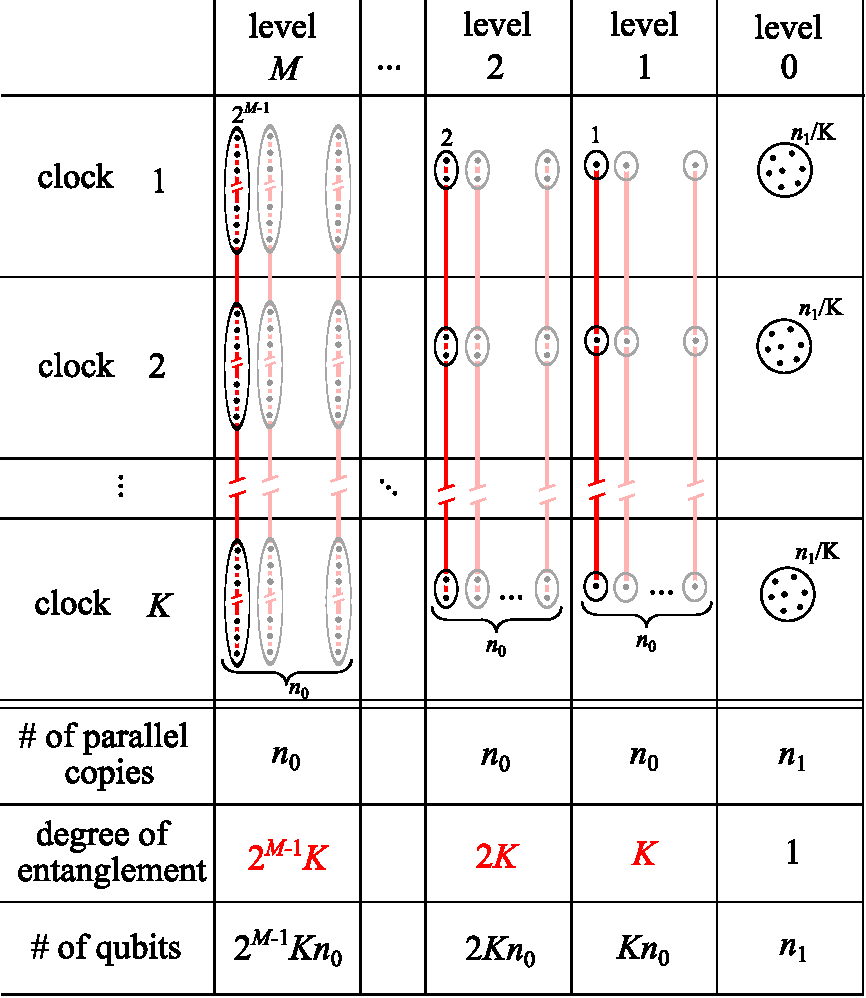
\includegraphics[width=0.8\textwidth]{./figs_Komar2014/fig_supp.pdf}  
\caption
[GHZ cascade protocol for $K$ clocks] 
{
\label{fig:GHZ_cascade}
GHZ cascade protocol for $K$ clocks. Each allocates qubits for different levels
of the protocol: In level 0, $n_1/K$ qubits are put into an uncorrelated
ensemble. In level $i$, $(i=1,2\dots M)$, each clock allocates $n_0 2^{i-1}$
qubits for creating $n_0$ parallel instances of GHZ states with $2^{i-1}K$
entangled qubits. Due to the exponential scaling of the degree of entanglement, most of
the total available qubits are used in higher levels of the cascade. This is a
necessary condition to achieve Heisenberg scaling, up to logarithmic factors.}
\end{figure}
  
The purpose of this cascaded scheme is to directly assess the digits $Y_1$ and
$\{Z_j\,:\, j=2,3,\dots\}$ in the binary fraction representation of the phase
\bel
	\Phi_\mathrm{LO}\mod[-\pi,\pi] = \frac{2\pi}{K}\left[Y_1 +\sum_{i=1}^\infty
	Z_{i+1}/2^i\right] - \pi,
\eel
where $x \mod [-\pi, \pi] = (x+\pi) \mod 2\pi - \pi$, $Y_1\in\{0,1,2\dots K-1\}$
and $Z_i\in\{0,1\}$, and $\Phi_\mathrm{LO} = \Phi_\mathrm{COM}$. The $0$th level of
the cascade estimates $\Phi_0 =
\sum_{j=1}^K \left(\Phi^{(j)}\mod[-\pi,\pi]\right)/K$, and every $i$th
level after that estimates $\Phi_i = K2^{i-1}\Phi_\mathrm{LO} \mod [-\pi,\pi]$. 
In other words, every level of the cascade is sensitive to a different
multiple of the LO phase $\Phi_\mathrm{LO}$ ($\mathrm{mod}\; 2\pi$). After the
separate measurements of the levels, each provide an estimate to $\Phi_i$ which
can be combined to obtain the best estimate for $\Phi_\mathrm{LO}$. Here we
describe this using the digits $Y_1$ and $Z_i$ as intermediate quantities,
which are calculated from $\Phi_i$ the following way,
% 
% By choosing an appropriate Ramsey time $T$, we can make
% sure that the phase of the $0$th level is slipping at a sufficiently slow rate,
% we can allow entangling $K$ qubits together in group $i=1$, since if their phase
% $\Phi_1$ wraps around $2\pi$, we can detect this by checking if the estimate
% $\Phi_0^\mathrm{est}$ from group $i=0$ is outside $[-\pi/K, \pi/K]$.
% 
% By continuing the same idea, the number of phase wraps in group $i$, $Z_i$, can
% be estimated from the measured phase of group $i-1$, $\Phi^\mathrm{est}_{i-1}$ as
\bal
	Y_1 &=& \left[K(\Phi_0 + \pi) - (\Phi_1 + \pi)\right]/(2\pi),
	\\
	Z_i &=& \left[2(\Phi_{i-1} + \pi) - (\Phi_i + \pi)\right]/(2\pi),
\eal 
for $i=2,3, \dots M$. 
% Then, by using the measurement results from group
% $i$, we can get an estimate on $\tilde\Phi_i$ (since qubit measurements
% can detect phase only up to $2\pi$ shifts), which added with the number of phase
% slips results in the total estimate of $\Phi_i$:
% \bel
% 	\Phi_i^{\mathrm{est}} = \tilde\Phi_i^\mathrm{est} + 2\pi Z_i.
% \eel
% During a single cycle, all levels of the cascade provide phase
% information, which is processed successively starting from $i=0$, with the
% choice $Z_0^\mathrm{est} = 0$, and estimating all phases $\Phi_i^\mathrm{est}$, up
% to $i=M$.


The last group ($i=M$) contains GHZ states with the most entangled qubits.
These are the ones with the fastest evolving phase, and therefore they provide
the best resolution on $\Phi_\mathrm{LO}$. Since
there are $n_0$ independent instances, their phase $\Phi_{M} = 2\pi \sum_{i=1}^\infty Z_{M+i}/2^i$ is known
up to the uncertainty, $\ev{\Delta\Phi^2_{M}}_\mathrm{pr} =
\frac{1}{n_0}$, 

Assuming that all lower digits $\{Y_1,Z_j|j=2\hdots M \}$ have been determined correctly, this results in the total measurement uncertainty for $\Phi_\mathrm{LO}$:
\bel
	\label{eq:projection_GHZ 2}
	\ev{\Delta\Phi^2_\mathrm{LO}}_\mathrm{pr} =
	\frac{\ev{\Delta\Phi^2_{M}}_\mathrm{pr}} {(2^{M-1}K)^2} = \frac{4n_0}{N^2},
\eel
where, for the moment, we neglected individual qubit noise and assumed
$\Phi_\mathrm{LO}\in[-\pi,\pi]$.
However, in general, the estimation of the lower digits will not be perfect. In
the following section we investigate the effect of these \textit{rounding
errors} on the final measurement accuracy. From this analysis we find the
optimal number of copies $n_0$ and $n_1$.

\subsection{Rounding errors}
Whenever $|\Phi_0^\mathrm{est} - \Phi_0| > \pi/K$, or
$|\Phi_i^\mathrm{est} - \Phi_i| > \pi/2$ (for $i \geq 1$), we make a mistake by
under- or overestimating the number of phase slips $Y_1$ or $Z_{i+1}$,
respectively. To minimize the effect of this error, we need to optimize how the
total of $N$ qubits are distributed among the  various levels of the cascade. In
other words we need to find $n_{0,\mathrm{opt}}$ and $n_{1,\mathrm{opt}}$.

The probability that a rounding error occurs during the estimation of $Z_{i+1}$
is
\bel
	\PP_{i,\mathrm{re}} = 2\intop_{\pi/2}^\infty \d{\phi}
	\rho_i(\phi + \Phi_i) \leq 2\intop_{\pi/2}^\infty \d{\phi} \frac{1}{s_i^3}
	\exp\left[-\frac{\phi^2}{2s_i^2}\right]
\eel
where $\phi = \Phi_i^{\mathrm{est}} - \Phi_i$, and $\rho_i$ is the conditional
density function of $\Phi_i^\mathrm{est}$ for a given real $\Phi_i$, and $s_i^2 =
\mathrm{Var}(\Phi_i^\mathrm{est} - \Phi_i) = 1/n_0$ for $i\geq 1$, and $s_0^2 =
\ev{\Delta\Phi_0^2}_\mathrm{pr} = \frac{1}{K^2}\sum_{j=1}^K
\ev{(\Delta\Phi^{(j)})^2}_\mathrm{pr} = 1/n_1$, since
$\ev{(\Delta\Phi^{(j)})^2}_\mathrm{pr} = \frac{K}{n_1}$ for all $j$.
The upper bound for $\rho_i$ is obtained 
% under the assumption
% $\gamma_\mathrm{LO}/\gamma_\mathrm{ind} \gg N/n_0$ (so that the projection noise is
% the dominant noise term) 
by using the following upper bound for any binomial
distribution: ${n\choose k}p^k(1-p)^{n-k} \leq
\exp\left[-n\left(\frac{k}{n}-p\right)^2\right]$. (For details, see
Appendix \ref{app:Kessler2014}.)  The resulting probabilities, after
dropping the higher order terms in the asymptotic expansions, are
\bal
	\PP_{0,\mathrm{re}} &\approx& \frac{2K}{\pi} n_1^{1/2}
	\exp\left[-\frac{n_1\pi^2}{2K^2}\right],
	\\
	\PP_{i,\mathrm{re}} &\approx& \frac{4}{\pi} n_0^{1/2}
	\exp\left[-\frac{n_0\pi^2}{8}\right]\qquad (i\geq 1).
\eal
These approximate formulas are valid for $n_0 \geq 5$, as we have checked
numerically.

The phase shift imposed on the estimate of $\Phi_\mathrm{LO}$ by a
manifested rounding error of $Y_1$ is $2\pi/K$ and of $Z_{i}$ is $2\pi/
(K 2^{i-1})$, for $i=2,3\dots M$.
This
results in the total variance contribution,
\bel
	\ev{\Delta\Phi^2_\mathrm{LO}}_\mathrm{re} 
	=\left(\frac{2\pi}{K}\right)^2\left[\PP_{0,\mathrm{re}} +
	\sum_{i=2}^{M}\PP_{i-1,\mathrm{re}} (2^{-i+1})^2\right]
	\approx\left(\frac{2\pi}{K}\right)^2
	\left[\PP_{0,\mathrm{re}} +
	\frac{1}{3}\PP_{i-1,\mathrm{re}}\right].
\eel
We simplify this expression by choosing $n_1$ so that  $\PP_{0,\mathrm{re}}
\approx \frac{2}{3} \PP_{i,\mathrm{re}}$:
\bel
	n_1 = \alpha K^2 n_0,
\eel
where $\alpha \approx \mathrm{max}\left\{1\;,\; \frac{2}{\pi^2 n_0}
\log\left(3K^2\frac{\sqrt{8}}{\pi n_0^{1/2}}\right)\right\} \ll n_0,
K$.
With this choice, we can write the rounding error contribution as
\bel
	\label{eq:Rounding_GHZ 2}
	\ev{\Delta\Phi^2_\mathrm{LO}}_\mathrm{re} \approx \frac{16\pi}{K^2}
	n_0^{1/2} \exp\left[-\frac{n_0 \pi^2}{8}\right].
\eel
We note that the amount of extra resources needed for the 0th level is
marginally small, since the total qubit number can be expressed as
\bel
	N = n_1 + n_0 K \sum_{i=1}^M 2^{i-1} = n_0 K(\alpha K + 2^{M} -2) \approx
	n_0 K2^{M},
\eel
under the assumption $K \ll 2^{M}$.

By adding the two error contributions from \refeq{eq:projection_GHZ 2} and
\refeq{eq:Rounding_GHZ 2}, we obtain the corresponding Allan-variance 
in the stationary noise approximation,
\bal
	\sigma_y^2(\tau) &=& \frac{1}{\omega_0^2 \tau T} \ev{\Delta\Phi_\mathrm{LO}^2}   
	=:
	\frac{1}{\omega_0^2\tau}\left[\Gamma_1 + \Gamma_2\right] =\\	
	&=& \frac{1}{\omega_0^2\tau}\left[\frac{4n_0}{N^2 T} +
	\frac{16\pi}{K^2 T} n_0^{1/2}\exp\left[-\frac{n_0\pi^2}{8}\right] 
	\right]
\eal
Now, let us find the optimal value of $n_0$. We write $\Gamma_1 + \Gamma_2$,
using the new variable $x = \frac{8}{\pi^2}\frac{1}{n_0}$, as
\bel
	\Gamma_1 + \Gamma_2 = \frac{4}{T}\left(\frac{8}{\pi^2}\frac{1}{x N^2} +
	\frac{\sqrt{32}}{K^2}\frac{1}{x^{1/2}}\exp\left[-\frac{1}{x}\right]\right).
\eel
Taking the derivative with respect to $x$ and equating it with 0, while using
the assumption $x \ll 1$ results in $\Gamma_2 \approx
x_\mathrm{opt}\Gamma_1 \ll \Gamma_1$, which can be written as the
following transcendental equation for the optimal value, $x_\mathrm{opt}$,
\bel
	x_\mathrm{opt}^{1/2} \approx 
	\frac{\pi^2N^2}{\sqrt{8}K^2}\exp\left[-\frac{1}{x_\mathrm{opt}}\right].
\eel
The general solution of any equation of the form $x^\nu = A \exp[-1/x]$, in the
limit of $A \gg 1$ and $x \ll 1$, is $x = [\log(A)]^{-1}$ . (For details, see
Appendix \ref{app:Kessler2014}.) Using this result we can write
\bal
	x_\mathrm{opt} &\approx&
	\left[\log\left(\frac{\pi^2}{\sqrt{8}}\frac{N^2}{K^2}\right)\right]^{-1} \sim
	[2\log(N/K)]^{-1}
	\\
	n_{0,\mathrm{opt}} &\approx&
	\frac{8}{\pi^2}\frac{1}{x_\mathrm{opt}} \sim \left(\frac{4}{\pi}\right)^2
	\log\left(N/K\right).
\eal
For the realistic case of $N/K \gg 1$, indeed $x_\mathrm{opt} \ll 1$, and the
corresponding minimal value of $\Gamma_1 + \Gamma_2$ is
\bel
	\label{eq:Gamma_1 + Gamma_2 min}
	[\Gamma_1 + \Gamma_2]_\mathrm{min} \approx \Gamma_1(x_\mathrm{opt}) =
	\left(\frac{8}{\pi}\right)^2\frac{\log(N/K)}{N^2 T}.
\eel
This result indicates that, in terms of qubit number, only a
logarithmic extra cost is required to achieve the Heisenberg limit. 

\subsection{Phase slip errors}
Although the cascade is designed to detect phase slips of all levels $i=1,2\dots
M$, a possible phase wrap of level $i=0$ remains undetected. Since the
qubits at different clocks are interrogated independently on the $0$th
level, each of them estimates the phase of the corresponding LO, $\Phi_0^{(j)}$
($j=1,2, \dots K$), and not $\Phi_\mathrm{LO}$, the phase accumulated by the
local oscillator.
The probability of $\Phi_0^{(j)}$ falling outside the interval $[-\pi,\pi]$ at least once during the total
measurement time $\tau$ is
\bal
	\PP_{j,\mathrm{slip}} &=& 2\frac{\tau}{T} \intop_\pi^{\infty}\d{\phi}
	\frac{1}{\sqrt{2\pi\gamma_\mathrm{LO}
	T}}\exp\left[-\frac{\phi^2}{2\gamma_\mathrm{LO}T}\right] \approx 
	\nonumber\\
	&\approx&
	\frac{\tau}{T}\frac{\sqrt{2}}{\pi^{3/2}}\sqrt{\gamma_\mathrm{LO}T}
	\exp\left[-\frac{\pi^2}{2\gamma_\mathrm{LO}T}\right],
\eal
where $\gamma_\mathrm{LO}$ is the linewidth of the local oscillator at clock $j$,
corresponding to a white noise spectrum, resulting in a constant phase 
diffusion over the interrogation time $T$, (which is assumed to be
approximately equal to the cycle time). The approximate form above is obtained
by neglecting the higher order terms in the asymptotic series expansion under the
assumption $\gamma_\mathrm{LO}T \ll 1$. 
(The white noise assumption can be relaxed to include more realistic LO
noise spectra.
However, numerical simulations have shown that, for a LO subject to a feedback
loop, the low frequency noise is essentially white even though the LO may have
more complicated noise spectrum, such as 1/f noise. Therefore the results
derived for white noise applies up to a constant prefactor.
\cite{Borregaard2013} We proceed with the white noise assumption for
simplicity.) Once such a phase slip happens, it
introduces a $2\pi$ phase shift in $\Phi_0^{(j)}$, and therefore contributes to
its overall uncertainty with $\ev{(\Delta\Phi_0^{(j)})^2} = (2\pi)^2
\PP_{j,\mathrm{slip}}$. Physically $\Phi_0$ is the phase of the COM signal, that
the center can obtain after averaging the frequencies of all $K$ local
oscillators with equal weights, $\Phi_0 = \Phi_\mathrm{COM} = \sum_{j=1}^K
\Phi_{0}^{(j)}/K$, therefore
$
	\ev{\Delta\Phi_0^2} = \frac{1}{K^2}\sum_{j=1}^K \ev{(\Delta\Phi_0^{(j)})^2} =
	\frac{1}{K}\ev{(\Delta\Phi_0^{(j)})^2},
$
where we assumed that the LOs are independent but they have the same linewidth,
$\gamma_\mathrm{LO}$. Therefore the noise of the COM phase is reduced
compared to the individual LOs. Since $\Phi_0 = \Phi_\mathrm{LO}$, the above
results in the following variance contribution
\bel
	\label{eq:Slip_GHZ 2}
	\ev{\Delta\Phi^2_\mathrm{LO}}_\mathrm{slip} =
	\sqrt{32\pi} \frac{\tau \gamma_\mathrm{LO}^{1/2}}{T^{1/2} K}
	\exp\left[-\frac{\pi^2}{2\gamma_\mathrm{LO}T}\right].
\eel
After adding this error to the previously minimized projection and rounding
error terms (from \refeq{eq:Gamma_1 + Gamma_2 min}), we obtain the corresponding
Allan-variance, $\sigma_y^2(\tau) =\frac{1}{\omega_0^2\tau}\left([\Gamma_1 + \Gamma_2]_\mathrm{min} +
\Gamma_3\right)$, where 
% \bel 
% 	\Gamma_3 = \sqrt{32\pi} \frac{\tau \gamma_\mathrm{LO}^{1/2}}{T^{3/2}K}
% 	\exp\left[-\frac{\pi^2}{2\gamma_\mathrm{LO}T}\right].
% \eel
\bel
	[\Gamma_1 + \Gamma_2]_\mathrm{min} + \Gamma_3 =
	\left(\frac{8}{\pi}\right)^2
	\frac{\log(N/K)}{N^2}\frac{2\gamma_\mathrm{LO}}{\pi^2}\frac{1}{y} +
	\frac{16}{\pi^{5/2}}\frac{\tau\gamma_\mathrm{LO}^2}{K}\frac{1}{y^{3/2}}
	\exp\left[-\frac{1}{y}\right],
\eel
using the variable $y = \frac{2}{\pi^2}\gamma_\mathrm{LO}T$. 

Now, let us find the optimal
Ramsey time $T_\mathrm{opt}$, under the assumption that $\tau$ is sufficiently
long.
After taking the
derivative with respect to $y$ and equating it with zero, the assumption $y_\mathrm{opt}\ll
1$ results in the $\Gamma_3 \approx y_\mathrm{opt}[\Gamma_1 +
\Gamma_2]_\mathrm{min} \ll [\Gamma_1 +
\Gamma_2]_\mathrm{min}$ which can be written as the following transcendental
equation,
\bel
	y_\mathrm{opt}^{3/2} \approx
	\frac{\pi^{3/2}}{8}\frac{\tau\gamma_\mathrm{LO}}{K}\frac{N^2}{\log(N/K)}
	\exp\left[-\frac{1}{y}\right].
\eel
The asymptotic solution in case of $y_\mathrm{opt}\ll 1$ is (see Appendix
\ref{app:Kessler2014})
\bal
	y_\mathrm{opt} &\approx&
	\left[\log\left(\frac{\pi^{3/2}}{8}\frac{\tau
	\gamma_\mathrm{LO}}{K}\frac{N^2}{\log(N/K)}\right)\right]^{-1},
	\\
	\label{eq:T_op_GHZ 2}
	T_\mathrm{opt} &\approx& \frac{\pi^2}{2}\frac{y_\mathrm{opt}}{\gamma_\mathrm{LO}}
	\sim
	\frac{\pi^2}{2\gamma_\mathrm{LO}}\left[\log(\tau\gamma_\mathrm{LO}N^2/K)\right]^{-1}
\eal
in the realistic limit of $\gamma_\mathrm{LO}\tau N^2/K \gg 1$. The corresponding
minimal Allan-variance is
\bel
% 	[\Gamma_1 + \Gamma_2]_\mathrm{min}(y_\mathrm{opt}) =
% 	\\
% 	&&\qquad =
	\label{eq:long_tau}
	\sigma_y^2(\tau) = \frac{1}{\omega_0^2\tau}\Big[[\Gamma_1 +
	\Gamma_2]_\mathrm{min} + \Gamma_3\Big]_\mathrm{min} \approx
	\frac{1}{\omega_0^2}\frac{L\gamma_\mathrm{LO}}{N^2 \tau},
\eel
where $L =
\frac{128}{\pi^4}\log(N/K)\log(\tau\gamma_\mathrm{LO}N^2/K)$.

For short $\tau$ averaging times, the optimal Ramsey time is
$T_\mathrm{opt}=\tau$, instead of \refeq{eq:T_op_GHZ 2}. This makes $\Gamma_3$
negligible compared to $[\Gamma_1 + \Gamma_2]_\mathrm{min}$, resulting in a
$1/\tau^2$ scaling:
% As an approximation, we obtain the total Allan-variance by
% adding the two expressions, $\sigma_y^2(\tau) \approx
% \frac{1}{\omega_0^2 \tau}([\Gamma_1 + \Gamma_2]_{n_0 =
% n_{0,\mathrm{opt}},T=\tau} + [[\Gamma_1 + \Gamma_2]_{n_0 =
% n_{0,\mathrm{opt}}} +
% \Gamma_3]_{T=T_\mathrm{opt}} + \Gamma_4)$.
\bal
	\label{eq:short_tau}
	\sigma_y^2(\tau)=\frac{1}{\omega_0^2\tau}[\Gamma_1 +
	\Gamma_2]_\mathrm{min}^{T=\tau} = \frac{1}{\omega_0^2}\frac{L'}{N^2 \tau^2}.
\eal
where $L' = \left(\frac{8}{\pi}\right)^2 \log(N/K)$. This scaling is more
favorable, but it applies to higher $\tau$ values up to $\tau \sim
\gamma_\mathrm{LO}^{-1}$, where it switches to the $1/\tau$ behavior according to
\refeq{eq:long_tau}.
%  and $L = L'
% \frac{2}{\pi^2}\log(\gamma_\mathrm{LO}\tau N^2/K)$.
% This result shows that
% for increasing $N$, the first two terms slowly diminishes with respect to the
% individual qubit noise. This is due to the quantum enhancement of the GHZ state.

\subsection{Pre-narrowing the linewidth}
We can minimize the limiting effect of $\gamma_\mathrm{LO}$ by narrowing the
effective linewidth of the local oscillators beforehand. We imagine using $N\s$
qubits to locally pre-narrow
the linewidth of all LOs down to an effective linewidth $\gamma_\mathrm{eff} \sim
\gamma_\mathrm{ind}N$, before using the remaining $N-N\s$ qubits in the GHZ
cascade.
This $\gamma_\mathrm{eff} \ll \gamma_\mathrm{LO}$ allows the optimal Ramsey time
going above the previous limit, set by $\sim \gamma_\mathrm{LO}^{-1}$ in
\refeq{eq:T_op_GHZ 2}.
This step-by-step linewidth narrowing procedure, using uncorrelated ensembles in
every step, is introduced in \cite{Rosenband2013,Borregaard2013}, and
further analyzed in \cite{Kessler2014}. Working under the small $N\s$
assumption, one can obtain $\gamma_\mathrm{eff}$ as
\bel
	\gamma_\mathrm{eff} \approx 
	\gamma_\mathrm{LO}\left[\frac{2}{\pi^2}\frac{\log(\gamma_\mathrm{LO}\tau
	n)}{n}\right]^{N\s/n},
\eel
where we imagine using $n$ qubits in each narrowing step. We find the optimal
value of $n$ to be
\bel
	n_\mathrm{opt} \approx \frac{2e}{\pi^2}\log(\gamma_\mathrm{LO}\tau),
\eel 
by minimizing $\gamma_\mathrm{eff}$, which yields
\bel
	\label{eq:gamma_m2}
	[\gamma_\mathrm{eff}]_\mathrm{min} \sim \gamma_\mathrm{LO}\exp\left[-\frac{N\s
	\pi^2}{2e\log(\gamma_\mathrm{LO}\tau)}\right].
\eel

For a given $\tau$, we can always imagine carrying out this pre-narrowing, so
that $\gamma_\mathrm{eff} < \tau^{-1}$, and therefore \refeq{eq:short_tau} remains
valid with the substitution $N\mapsto N-N\s$ for $\tau >
\gamma_\mathrm{LO}^{-1}$ as well. The required number of qubits, $N\s$, is
\bel
	N\s \sim
	\frac{2e}{\pi^2}\log(\gamma_\mathrm{LO}\tau)
	\log\left(\frac{\gamma_\mathrm{LO}}{\gamma_\mathrm{ind}N}\right) \ll N.
\eel
due to the exponential dependence in \refeq{eq:gamma_m2}.


\subsection{Individual qubit dephasing noise}
Our scheme, as well as any scheme, is eventually limited by individual qubit
noise. Such a noise dephases GHZ states at an increased rate, compared to
uncorrelated qubits, due to the entanglement, giving the corresponding variance
contribution for the phase of the GHZ states in the $M$th group, 
$\ev{\Delta\Phi^2_{M}}_\mathrm{dephasing} =  \frac{2^{M-1}
K\gamma_\mathrm{ind}T}{n_0}$, after averaging over the $n_0$ independent copies of the GHZ states, each
containing $2^{M-1} K$ entangled qubits. The resulting variance
contribution for $\Phi_\mathrm{LO}$ is
\bel
	\label{eq:Dephasing_GHZ 2}
	\ev{\Delta\Phi^2_\mathrm{LO}}_\mathrm{dephasing} =
	\frac{ \gamma_\mathrm{ind}T}{n_0 2^{M-1}K} = \frac{2\gamma_\mathrm{ind}T}{N}.
\eel
This term represents a noise floor, which we add to
\refeq{eq:short_tau} and obtain our final result for the minimal achievable
Allan-variance,
\bel
	\label{eq:Final sigma_y}
	\sigma_y^2(\tau) = \frac{1}{\omega_0^2}\left[\frac{L'}{N^2 \tau^2} +
	\frac{2\gamma_\mathrm{ind}}{N\tau}\right].
\eel

For long $\tau$ times, the ultimate limit, set by the standard quantum limit,
$
	\sigma_y^2(\tau) = \frac{1}{\omega_0^2}
	\frac{\gamma_\mathrm{ind}}{N\tau},
$
can be reached by changing the base of the cascade. Instead of entangling
2-times as many qubits in each level of the cascade than in the previous level,
we imagine changing it to a base number $D$. Carrying out the same calculation
results in our final result for the achievable Allan-variance:
\bel
	\sigma_y^2(\tau) =
	\frac{1}{\omega_0^2}\left[\left(\frac{D}{2}\right)^2\frac{L'}{N^2 \tau^2} +
	\frac{D}{D-1}\frac{\gamma_\mathrm{ind}}{N\tau}\right],
\eel
where $L' = \left(\frac{8}{\pi}\right)^2 \log(N/K)$.
(See Appendix \ref{app:Kessler2014} for details.)
The optimal value of $D$ depends on $\tau$. For small $\tau$, $D_\mathrm{opt} =
2$, however for large $\tau$ one can gain a factor of 2 by choosing $D_\mathrm{opt} = D_\mathrm{max}$. Due to natural
constraints, $D_\mathrm{max} \sim \sqrt{N}$, in which regime, the protocol
consists of only two cascade levels, an uncorrelated 0th level, with $\sim
\sqrt{N}$ qubits and an entangled 1st level with $\sim N$ qubits.

% \#\#\#\#\#\#\#\#\#\#\#\#\#\#\#\#\#\#\#\#\#\#\#\#\#\#\#\





\section{Security countermeasures}

\subsection{Sabotage}
In order to detect sabotage, the center can occasionally perform assessment
tests of the different nodes by teleporting an uncorrelated qubit state $[\ket{0} +
e^{i\chi}\ket{1}]/\sqrt{2}$, where $\chi$ is a
 randomly chosen phase known only to the center.
A properly operating node creates a local GHZ state $[\ket{\mathbf{0}} +
e^{i\chi}\ket{\mathbf{1}}]/\sqrt{2}$ from the sent qubit,
 measures the parity of the GHZ state, and sends it to the center. The
measured parity holds information on the phase $\phi' = \chi + \phi$, where
$\phi$ is the accumulated phase of the LO at the node. Due to the random shift
$\chi$, this appears to be random to the node, and therefore indistinguishable
from the result of a regular (non-testing) cycle. On the other hand, the center
can subtract $\chi$, and recover $\phi$ from the same measurement results. In
the last step, the center verifies $\phi$ by comparing it with the classically
determined phase $\phi_\mathrm{cl}$ of the sent LO signal with respect to the COM
signal. The expected statistical deviation of
$\phi$ from $\phi_\mathrm{cl}$ is $\Delta(\phi -
\phi_\mathrm{cl})\sim\sqrt{\frac{K}{N}}$, while the accuracy of the COM phase
$\Delta(\phi_\mathrm{COM} - T\omega_0)\sim\sqrt{\frac{K}{(K-K_t)N}}$ is much
smaller, where $K_t$ is the number of simultaneously tested nodes. In the likely
case of $K_t \ll K$, this method is precise enough for the center to
discriminate between healthy and unhealthy nodes by setting an acceptance range,
$|\phi - \phi_\mathrm{cl}| \leq \Lambda \sqrt{\frac{K}{N}}$. E.g. the choice of
$\Lambda = 4$ results in a ``$4\sigma$ confidence level'', meaning only 0.0063\%
chance for false positives (healthy node detected as unhealthy), and similarly
small chance for false negatives (unhealthy node being undetected)
$(\sim\Lambda\frac{\Delta \phi'}{2\pi}\propto 1/\sqrt{N}) $ due to the high
precision with which $\phi'$ is measured.
The fact, that the teleported qubit can be measured only once, also prevents the
nodes from discovering that it is being tested. In fact the
center performs a very simple blind quantum computing task using the resources
of the other clocks, see \cite{Childs2001, Broadbent2009, Mantri2013}.

\subsection{Eavesdropping}
Provided that the threat of sabotage is effectively eliminated, we turn our
attention to the problem of eavesdropping. Eavesdroppers would try to intercept
the sent LO signals, and synthesize the stabilized $\nu_\mathrm{COM}$ for themselves. Our
protocol minimizes the attainable information of this strategy by prescribing
that only the \emph{non-stabilized} LO signals are sent through classical
channels. This requires the feedback to be applied to the LO signal after some
of it has been split off by a beam splitter, and the center to integrate the
generated feedback in time. Alternatively, eavesdroppers could try intercepting
the LO signals \emph{and} the feedback signals, and gain access to the same
information, the center has. This can be prevented by encoding the radio
frequency feedback signal with phase modulation according to a shared secret
key. Since such a key can be shared securely with quantum key distribution, this protocol keeps the feedback signal hidden from outsiders. As a
result, even the hardest-working eavesdropper, who intercepts all LO signals, is
able to access only the non-stabilized COM signal, and the stabilized COM signal
remains accessible exclusively to parties involved in the collaboration.

\subsection{Rotating center role}
Since the center works as  a hub for all information, ensuring
its security has the highest priority. In a scenario,  where 
a small number of nodes (without knowing which) cannot be 
trusted enough to play the permanent role of the center, a rotating stage
scheme can be used. By passing the role of the center around, the
potential vulnerability of the network due to one untrustworthy site is
substantially lowered. This requires a fully connected
network and a global scheme for assigning the role of the center.


\section{Network operation}

\subsection{Different degree of feedback}
Apart from the full feedback, described in the main text, alternatively, the
center can be operated to provide restricted feedback information to the nodes.
If the center sends the averaged error signal $\tilde \delta_\mathrm{COM}$ only,
the LOs at the nodes will not benefit from the enhanced stability and only the
center can access the stabilized signal. Of course the LO at each node will have
its own local feedback to keep it within a reasonable frequency range around the
clock transition. Such a 'safe' operational mode allows the center node to
use the resources of other nodes, while keeping the world time signal hidden
from them. Such an asymmetric deal can be incentivized by monetary compensation,
and allow the inclusion of nodes that cannot be trusted to keep the time signal
secret.

As an intermediate possibility, the center can choose to send regionally
averaged feedback signals $\tilde\delta_\mathrm{COM} + \sum_{j\in R}(\nu_j -
\nu_\mathrm{COM})/|R|$, uniformly for all $j\in R$ nodes, where $R$ is a set of
nodes, ie. a region. Such a feedback scheme creates the incentive of cooperation
for the nodes in region $R$. By properly sharing their LO signals with each
other, the nodes can synthesize the regional COM frequency, $\sum_{j\in
R}(\nu_j)/|R|$, and steer it with the feedback, received from the center.


\subsection{Timing}
Proper timing of local qubit operations is necessary to ensure that every qubit
in the network is subject to the same $T$ free evolution time.
The finite propagation time of light signals introduces delays in the quantum
links and classical channels.
Similarly, during the entangling step, the finite time required to do local
entangling operations make the free evolution start at slightly different times
for different qubits. Since both the initialization and the measurement are local
operations, we can resolve the issue of delay by prescribing that the
measurement of qubit $i_j$ ($i$th qubit at node $j$) takes place exactly $T$
time after its initialization. Occasional waiting times of known length can be
echoed out with a $\pi$-pulse at half time. 

In extreme cases, this might cause
some qubits to be measured before others are initialized. However, this is not a
problem, since the portion of the GHZ state that is alive during the
time in question is constantly accumulating the $\phi_j$ phases from the qubits
it consists of. This results in the phenomenon that the total time of phase accumulation can be much longer than the length of individual
phase accumulations, provided that the said interrogations overlap.

\subsection{Dick effect}
Classical communication between the clocks, separated by large geographical
distances, takes considerable time compared to the interrogation time. The
requirement to communicate the outcome of the Bell measurement in each
teleportation step results in a waiting time in the teleportation protocol.
During this waiting time (or dark time) the qubits are not interrogated, and
therefore the local oscillator runs uncontrollably. If not countered, this
effect (Dick effect) will deteriorate the overall stability of the clock
network.
Essentially the problem arises from the duty cycle of the clock being less than
100 percent. By employing two parallel realizations of the network scheme
(supported by the same clock stations, but using different qubits) whose cycles
are offset by half a period in time, we can cover the entire cycle time with at
least one copy of the clock network being interrogated at all times. As a
result, we can cancel the Dick effect with only a constant factor ($\sim 2$) 
increase in the required resources, if the required time to prepare and measure
the state is not longer than the free evolution.


\subsection{More general architectures}
So far, we focused on the simplest network structure with one center
initiating every Ramsey cycle and nodes with equal number of clock qubits.

In a more general setup, node $j$ has $N_j$ clock qubits. If $N_j$ is different
for different $j$, then the nodes will contribute the global GHZ states
unequally, resulting in entangled states which consists of different $N_j'$
number of qubits from each site $j$. Such a state picks up the phase
\bel
	\Phi = \sum_{j}N'_j \phi_j,
\eel
where $\phi_j$ is the phase of the LO at site $j$ relative to the atomic
frequency. As a result, the clock network measures the following collective LO
frequency
\bel
	\nu_\mathrm{LO} = \frac{\sum_{j}N'_j \nu_j }{ \sum_{j}N'_j}.
\eel
This represents only a different definition of the world time (a weighted
average of the times at the locations of the nodes, instead of a uniform
average), but it does not affect the overall stability.

The initial laser linewidths of the nodes $\gamma_\mathrm{LO}^j$ can also be
different. The stability achievable in this case is bounded by the stability
obtained for a uniform linewidth $\gamma_\mathrm{LO} = \max_j \gamma_\mathrm{LO}^j$.
If linewidths are known, the center can devise the best estimation method
which uses linewidth dependent weights in the LO frequency averaging step. 


Although it is simple to demonstrate the important network operational concepts
with the architecture with one center, this structure is not a necessary. The
quantum channels, connecting different nodes, can form a sparse (but still connected)
graph, and the entanglement global entanglement can still be achieved by
intermediate nodes acting as repeater stations. This way entanglement can be
passed along by these intermediate nodes. Moreover, the center can be eliminated
from the entangling procedure by making the nodes generate local GHZ states, and
connect them with their neighbors by both measuring their shared EPR qubit with
one of the qubits form the local GHZ state in the Bell-basis. After
communicating the measurement result via classical channels, and performing the
required single qubit operations, a global GHZ state is formed.


\subsection{Accuracy}
We define the accuracy of a time signal as the total uncertainty of its
frequency with respect to the fundamental time reference. This includes the
precision (characterized by the Allan deviation) and the uncertainty of
frequency shifts due to systematic effects. So far we analyzed only the
precision.

If two clocks have different levels of uncertainty for the local systematic
shifts, then their individual accuracy is different. Our scheme requires the
clocks to work together coherently, and thereby it averages out these
differences in accuracy sub-optimally. In order to determine the individual
accuracies, the clock network has to disentangle one of the clocks from the
others. Next, by comparing the time signal from the
entangled network with the one from the excluded clock, it can determine if the
said clock has higher or lower accuracy than the average. By rotating this
scheme, the systematic shifts of the worse clock can be measured more precisely,
and, on the long run, this results in an overall improvement of the accuracy.

Apart from the local systematic effects (such as blackbody shift, second order
Zeeman shift, etc.), a quantum network of clocks is subject to gravitational
redshifts, which affect clocks at different positions differently. In order to
ensure precise measurement of this systematic shift, the position of the clocks
has to be tracked with high precision. This can be done similarly to the way
ground stations track GPS satellites. The time signal generated
by the quantum clock network can be used to set up a more precise
tracking system, which can measure this systematics at a higher
accuracy.






\subsection{Efficient use of qubits}
In the main text, during the generation of the initial global GHZ state, we
assumed that the center makes use of $2(K-1)$ additional ancilla qubits ($a_j,
b_j$).
We chose this to present the idea at its simplest, however the qubits used as
ancillae do not have to be sitting uselessly during the interrogation time.
The center can use $2(K-1)$ out of its $N/K$ clock qubits to perform the local
generation and teleportation steps. This relabeling goes as follows $\{(b_j=
j_1,\; a_j=(K-1+j)_1)\;:\; j=2\dots K\}$.
After it is done, the qubits used as ancillae can be reinitialized, the center
can entangle the $2(K-1)$ qubits (alongside with the others) with $1_1$, and
interrogate them without any obstacles. As a result, no clock qubits are wasted
in the protocol.


\subsection{Required EPR generation rate}
 In the main text, we mainly ignored the time required to generate
 pairwise entanglement. In this section we investigate the required EPR
 generation rate to achieve the desired performance.
 Before every cycle of operation $n [\log(N/K)/\log(2) + 1] (K-1)$ EPR pairs
have to be shared between the center and the other clocks, where $n$ is the
number of parallel copies, $N$ is the total number of qubits in a single copy
and $K$ is the number of clocks.
Since $n_\mathrm{opt} \sim (4/\pi)^2 \log(N/K)$, and approximately $K$
quantum channels are used, the number of EPR pair per channel is about
$(\log(N))^2$. We can assume that entangled qubits can be stored in degenerate
memory states until they are used in the beginning of the next cycle. Therefore
each channel has $T$ time to initialize the $(\log(N))^2$ number of pairs. The
optimal value for $T$ is the available averaging time $\tau$, which we choose to
be $\sim 0.1\gamma_i^{-1}$ for order of magnitude estimation. (Note that $\tau <
\gamma_i^{-1}$ is required to benefit from quantum enhancement.) For $N=10^4$
atoms and $\gamma_i=2\pi \times 1 \;\mathrm{mHz}$, the EPR generation rate per
channel has to be at least $(\log(N))^2\gamma_i \sim 1\;\mathrm{Hz}$.
Such a rate is within reach of technology currently under intensive research 
\cite{monroe2014}.



\subsection{Threshold fidelity}
In this section we estimate the fidelity of the collective entangling operations
required to keep the benefit from quantum enhancement.
In the GHZ state generation step of every cycle, the $n$ copies of the cascaded
network containing $K$ clocks are initialized. This requires $K$ collective
entangling operations to be performed per level per copy, one at each clock.
Among other unitary operations, this is likely to be the bottleneck. If one
collective entangling operation (creating a GHZ state of $N/(Kn)$ qubits) can be
performed with fidelity $F = \exp[-\epsilon]$ $(\epsilon \ll 1)$, then $K$
repetitions succeed with fidelity $F_\mathrm{total} = F^{K}= \exp[-K\epsilon ]$.

Whenever a copy fails on level $i$, its measurement result $\phi_i$ becomes
completely random. This happens with probability
$(1-F_\mathrm{total})$.
In the meantime, with probability $F_\mathrm{total}$, the result is consistent with
$\phi_i = \phi_\mathrm{real}$, where $\phi_\mathrm{real}$ is the actual value of
$\phi_i $. Out of the $n$ copies $nF_\mathrm{total}$ contributes to a peak
centered at $\phi_\mathrm{real}$, with width of $1/\sqrt{F_\mathrm{total}n}$ and
weight $F_\mathrm{total}$, while the rest contributes to a uniform distribution
with weight $(1-F_\mathrm{total})$:
The expectation value of $\phi_i$ is still
\bel
 	\ev{\phi_i} = \phi_\mathrm{real},
\eel
but the variance is
 \bel
 	\mathrm{Var}(\phi_i) \approx \frac{1}{n} +
 	\frac{\pi^2}{3}(1-F_\mathrm{total}).
 \eel 
The threshold fidelity $F_\mathrm{th}$ is defined by the criteria that if $F \geq
F_\mathrm{th}$, then $\mathrm{Var}(\phi_i) \approx 1/n$. If this is satisfied, then
losing the information from some of the copies does not deteriorate
 the precision significantly with which $\phi_i$ can be determined .

This requires $1-F_\mathrm{total} < \frac{3}{\pi^2 n}$, where the optimal value
for $n$ is $n_\mathrm{opt}\sim \left(\frac{4}{\pi}\right)^2\log(N/K)$, while
$F_\mathrm{total}= \exp[-\epsilon K]$ from above. From these, we conclude that $F_\mathrm{th} =
\exp[-\epsilon_\mathrm{th}]$, where
\bel
	\epsilon_\mathrm{th} \approx \frac{3}{16 K \log(N/K)} \sim \frac{1}{K \log (N)}.
\eel 
 Using $N=10^4$ qubits, distributed in 10 clocks  therefore requires
 $F_\mathrm{th} \approx 0.99$ fidelity level for the local entangling operation.
Using a multi-qubit entangling gate \cite{MSgate}, this operation can be
realized with current technology for fidelity $\sim 0.95$ and for
small number of ions ($\sim 5$). \cite{Monz2011} The errors in such operations
increases with $N$, making their realization more challenging. Namely, a 2-ion
GHZ state was produced with 0.993 fidelity in a trapped ion system
\cite{Benhelm2008}.
Currently the largest GHZ state of 14 ions was produced with 0.51 fidelity
\cite{Monz2011}.
